\section{Apparato sperimentale}\label{sec:apparato-sperimentale}
Il circuito che abbiamo realizzato è schematizzato in figura \ref{fig:circuito}.
Le porte logiche sono realizzate usando dei circuiti integrati e sono collegate tra di loro
in modo da rispettare lo schema.

\subsection{Schema del circuito (multiplexer)}\label{subsec:schema-circuito}
\begin{figure}[h]
\centering
    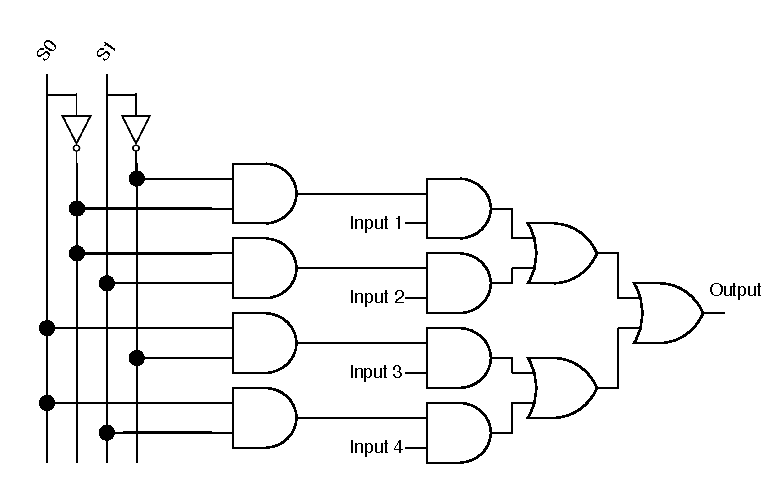
\includegraphics{../assets/circuito.drawio.pdf}
    \caption{
      \emph{
        Schema del circuito multiplexer. Le sigle sui gate indicano a quale circuito integrato corrispondono.
      }
    }
    \label{fig:circuito}
\end{figure}

\subsection{Materiale e strumenti usati}\label{subsec:materiali}
Segue una lista del materiale e degli strumenti usati per entrambi i circuiti durante la prova:
\begin{itemize}
  \item%
  Oscilloscopio analogico, modello: \emph{GW Instek GOS-652}.
  \item%
  Multimetro digitale, modello: \emph{ISO-TECH IDM 105}.
  \item%
  Generatore di tensione, modello: \emph{Aim-TTi EB2025T}.
  \item%
  Generatore di onda quadra, modello: \emph{GFG-8017G}.
  \item%
  Generatore di livelli logici, modello: \emph{Black Box}.
  \item%
  Sonda per oscilloscopio.
  \item%
  Connettori vari (connettori a banana, cavi per la scheda millefori).
  \item%
  Circuiti integrati per \textsc{or}, \textsc{and} (2x), \textsc{exor}, rispettivamente modelli: \emph{7432}, \emph{7408}, \emph{7404}.
\end{itemize}

\begin{table}[H]
  \centering
  \begin{tabular}[t]{c | c  c }
    \hline
    Grandezza & Valore & Fondoscala \\
    \hline
    d.d.p. generatore & $(5.03 \pm 0.03) \: V$ & $40 \: V$ \\
    Stato basso & $(0.0746 \pm 0.0012) \: V$ & $4 \: V$ \\
    Stato alto & $(3.92 \pm 0.04) \: V$ & $40 \: V$ \\
    \hline
  \end{tabular}
  \caption{\emph{Grandezze caratteristiche dei circuiti.}}
  \label{tab:livelli-logici}
\end{table}
